\documentclass[12pt]{article}
\usepackage[margin=0.5in]{geometry} 
\usepackage{amsmath,amsthm,amssymb,amsfonts,graphicx,subcaption}
\graphicspath {{images/}}
\usepackage{xcolor}

\usepackage{natbib}


\newcommand{\N}{\mathbb{N}}
\newcommand{\Z}{\mathbb{Z}}
 
\newenvironment{problem}[2][Problem]{\begin{trivlist}
\item[\hskip \labelsep {\bfseries #1}\hskip \labelsep {\bfseries #2.}]}{\end{trivlist}}
 
\begin{document}

\title{Computational Physics: Project Report\\\color{white}.\color{}\\ \textbf{Studying the Mechanics of Compressed Emulsions} }
\author{Aditya Vikram Hardikar \\ Supervisor : Jasna Brujic}
\maketitle

\begin{center}
  
\includegraphics[width = 0.3\linewidth]{images/nyu.jpeg}
\end{center}


%%%%%%%%%%%%%%%%%%%%%%%%%%%%%%%%%%%%%%%%%%
%%%%%%%%%%%%%%%%%%%%%%%%%%%%%%%%%%%%%%%%%%
%%%%%%%%%%%%%%%%%%%%%%%%%%%%%%%%%%%%%%%%%%
\begin{section}{Introduction}
Emulsions belong to the category of soft materials, whose properties are in between those of solids and fluids. Some examples of emulsions are mayonnaise, lotions whose physical properties are tweaked as required for usage. In this project, we study a system jammed particles specifically, compressed emulsion droplets\cite{brujic2004experimental} made of silicone oil and stabilized by as surfactant dispersed in an aqueous phase. We wish to study this system as it is an important model system used to study the jamming transition\cite{liu1998nonlinear}. These droplets aggregate to form a jammed structure given enough density. The droplets are visualized using confocal microscopy which returns a stack of images in different planes from which the positions of the centers and radii are computed.\cite{brujic2004experimental}. A pair of droplets in contact with each other interact via a normal force associated with the deformation of these squishy droplets.\\\\ 
We compute the forces on each of the droplets, which can be related to the deformation. In reality, this jammed system is in mechanical equilibrium. So, the sum of forces on each droplet must be zero. However, due to errors in the experimental imaging and analysis of the data, there is some residual force on each droplet. The objective is to find the corrected image of the emulsion hereby referred to as the 'relaxed' state of the system, where the residual force on each droplet is zero. This will be done using the method of steepest descent, to find the nearest minimum of the potential energy of the system. All of this is done with a view to study the vibrational modes of the system, once the relaxed state is known.
\end{section}
%%%%%%%%%%%%%%%%%%%%%%%%%%%%%%%%%%%%%%%%%%%
\begin{section}{Motivation}
The glass transition is said to occur when a material such as a polymer undergoes changes in physical properties when it is cooled below a certain temperature. It a problem of ongoing research to find out whether there is a phase transition underlying the glass transition. Similarly, when the density of particles in a system increases beyond a specific amount, physical properties of the system seem to undergo a phase transition. This is the so called mechanism of jamming which is similar to the glass transition, but also not well understood. The density at which jamming occurs is determined by several factors such as the sizes and shapes of the constituent particles, the forces in between the particles, temperature of the system. A jamming phase diagram has been proposed which tries to serve as a unifying link for these different transitions.\cite{liu1998nonlinear} \newline \newline
Some examples of systems that show jamming are emulsions or colloidal suspensions, granular material such as sand and structural glasses. With view to understand better the physical properties of jammed matter, we study the system of compressed emulsions, which are droplets of silicone oil dispersed in an aqueous phase. Beyond a certain density of emulsion droplets, the system is jammed and the physical properties of this are quite different from that of the liquid which it is made up of. For example, mayonnaise has properties which are neither fluid nor solid-like and the aim of our study is to understand this better. Specifically, we would like to calculate the vibrational modes of our compressed emulsion system. The procedure to do this, starting with the experimental setup is described in the following section.
\end{section}

\begin{section}{Procedure}

We wish to study the vibrational modes of our compressed emulsion with a view to understand jammed systems better. The system under consideration is a polydisperse emulsion of silicone oil droplets stabilized in an aqueous phase. We image the droplets using confocal microscopy and get a z-stack of 2D images. A typical image in the stack looks as following:
\begin{figure}[h!]
    \centering
    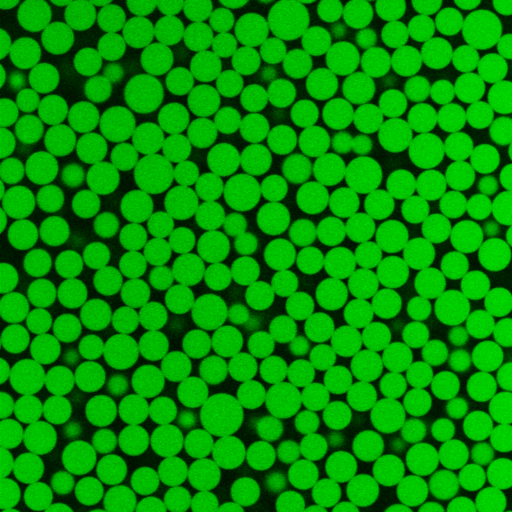
\includegraphics[width=0.5\linewidth]{emulsion_one_slice.png}
    \caption{Slice in the confocal image of the emulsion}
    \label{fig:my_label}
\end{figure}
\par \noindent An existing code matches the 3D image to a template sphere in Fourier space to return the positions of the centers and radii of these droplets. We start with the data of centers and radii of the droplets. Associated with two droplets overlapping, there is some deformation. This gives rise to a normal force along the line joining the centers of the droplets. Because the system is in a jammed state, a droplet experiences forces from several neighbouring droplets. We know that the net force on each droplet is zero, because the system is observed to be in mechanical equilibrium. Calculation of forces with the appropriate force model however, does not make the net force on each particle to be zero. This residual force error may arise due to one or more of the following reasons. 
\begin{enumerate}
    \item Shortcomings of the force model
    \item Errors in calculating the positions of the centers
    \item Errors in calculating the radii
\end{enumerate}
Assuming that errors arise due to errors from the centers and radii calculations, we want to write a program to correct for the positions of centers and radii of each droplet. Initially, we wish to correct the positions of the droplet centers and then if we succeed, we will try to correct the radii as well. The idea is to obtain the relaxed state of the system, which is the state where the net force on each droplet goes to zero. This can be done by implementing a gradient descent algorithm which minimizes the energy of the system. It is important to keep in mind that we want the \textbf{nearest minimum} of the system, as the relaxed state should be close to the original picture, since we know that the system has stabilized in such a manner. \\\\
Once the relaxed state is obtained, the idea is to do an expansion of the energy gradient around the minima to write the hessian matrix\cite{schindler2016range}, whose eigenvalues will give us the frequencies of the vibrational modes and the eigenvectors give the amplitudes of the droplets that are excited by the specific vibrational mode. The overall scheme is highlighted by the flowchart below. 
\begin{figure}[h!]
    \centering
    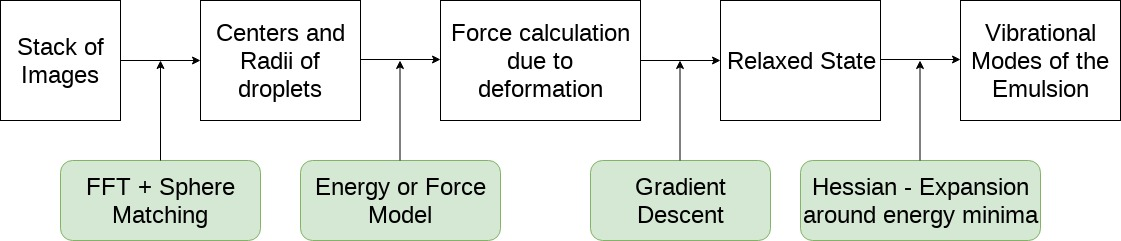
\includegraphics[width = 0.95\linewidth]{images/scheme.jpg}
    \caption{Flowchart of the process}
    \label{fig:my_label}
\end{figure}
\end{section}

%%%%%%%%%%%%%%%%%%%%%%%%%%%%%%%%%%%%%%%%%%%%%%%%
\newpage
\begin{section}{Theoretical Background}
    
\begin{subsection}{Batch Gradient Descent}
The gradient descent algorithm is particularly useful for searching for the extremum of a function where the landscape is unknown. For instance, in the case of our experimental data, we have around 1500 particles whose positions and radii contribute in a complex manner to determine the total energy of the sample. In other words, \begin{equation}
    U_{total} = f(\Vec{x_i}, r_i) 
\end{equation} where $\Vec{x_i}$ and $r_i$ are the position of the center and radii of the $i^{th}$ particle, and the index $i$ runs over all the droplets in the sample. The numerous minima of this function are hard to determine analytically, and thus we use the method of gradient descent or steepest descent. The physical analogy for this algorithm can be thought of as a ball rolling on a landscape, moving in the direction of the local slope it sees and settling down in a valley in the landscape. 
\\\\ 
The gradient descent begins by calculating the total potential energy of the current state that the system is in. In case of droplets interacting through a conservative force field which is the case with our force models, moving the droplets in the direction of the force, will take you to a lower potential energy. We calculate the force on each droplet and move the droplets in the direction of the force by a tiny amount given by the learning parameter $\alpha$. 
\begin{equation}
    \Vec{x}_{new,i} = \Vec{x}_{old,i} + \alpha \times \Vec{F_i}
\end{equation}
The alpha we choose is a small quantity, roughly $10^{-3}$ so that $\alpha \times \Vec{F}_i$ is of the order of $\frac{radius}{10^3}$. If the total energy of the system in the new configuration is less than the initial energy, that means we are moving in the direction of a local minimum and continue the process. The simultaneous update of the positions after checking this criterion is known as the batch gradient descent.  
\end{subsection}

\begin{subsection}{Gradient Descent with Momentum}
The gradient descent proceeds in small steps. To speed up this process we implement a gradient descent with momentum. Going back to the analogy of the ball rolling down the hill, we assign a velocity to the ball that it has gained from the previous iterations in the descent. This algorithm is known to converge faster to the local minimum and is quite robust. 
The algorithm proceeds as following
\begin{align}
    \Vec{x}_{new,i} &= \Vec{x}_{old,i} + \alpha \times \Vec{v}_{old,i} \\
    \Vec{v}_{new,i} &= \beta \times \Vec{v}_{old,i} + (1-\beta) \times \Vec{F_i}
\end{align}
The value of $\beta$ is chosen to be 0.9 \cite{qian1999momentum}, which is a widely used for for most situations. 
Although some cases implemented this algorithm, it was not used for the experimental data due to the possibility of many minima near each other, and we did not want to skip the nearest local minimum which we desire.
\end{subsection}

\begin{subsection}{Adaptive Step Size}
To ensure that we are not stuck in a sharp valley, we used an adaptive step by controlling the learning parameter $\alpha$. Whenever, the energy in the new configuration is greater than the energy in the previous configuration, instead of stopping the algorithm, we take a smaller value of alpha and try again so as to make a better approximation to the position of the minima
\end{subsection}

\begin{subsection}{Boundary Conditions}
We have a z-stack of images which are obtained from experiment. We do not know what lies outside the region of observation. We have some droplets in the sample on the edges of the figure whose neighbours are not known. Hence, we fix the positions of these droplets referred to as the \textbf{edge droplets} and do not calculate the residual forces on these droplets. For a poly-disperse system, we identify edge droplets as the ones that lie within distance $d_{max} = 2 \times r_{max}$ from the edges, which is the diameter of the particle with the maximum radius in the sample. All test cases also consider such boundary conditions.
\end{subsection}

\begin{subsection}{Interaction Model: Simple Harmonic Potential}
We primarily use two force models to model the interactions between our droplets which are treated as  deformable spheres. If the distance between the centers of two droplets is larger than the sum of there radii, that means there is no deformation, and there is no force. However, if the overlap $x$
\begin{equation}
    x = \text{Distance between centers} - \text{Sum of radii}
\end{equation}
is less than $0$, the force and the potential energy associated with the pair droplets is non-zero. 
For the simple harmonic potential, the deformation is considered to obey the Hooke's law, so that the force and potential are:
\begin{align}
    \Vec{F} &= -kx\hat{x} \\
    U &= \frac{1}{2} k x^2
\end{align}
This model is used as a simple check for whether the gradient descent works well and is used on the test cases.
\end{subsection}
\begin{subsection}{Interaction Model: Area-Dependent Potential (Princen Model)}
The deformable spheres are much more complex than a simple spring. A well known model \cite{princen1983rheology} that also takes polydispersity into consideration is the Princen model. This model associates the force between droplets with the area of the deformation as seen in figure below. The reson for doing this is that the change in energy is propotional to the interfacial tension $\sigma$ between the droplets times the change in area. 
\begin{figure}[h!]
    \centering
    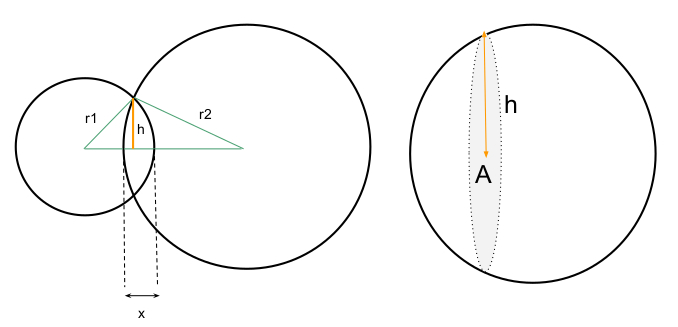
\includegraphics{area_potential.jpeg}
    \caption{Schematic for the area associated with droplet deformation}
    \label{fig:my_label}
\end{figure}
\par \noindent The area can be estimated as $\pi \times h^2$ where h is calculated by the area of the triangle formed by the green lines in the figure below using the Heron's formula.
\begin{equation}
    \text{area of green triangle} = \sqrt{(s)(s-r_1)(s-r_2)(s-(r_1+r_2-x)} =  \frac{1}{2}h(r_1 + r_2 -x)
\end{equation}
The force is given by
\begin{equation}
    \Vec{F} = -\frac{\sigma}{\Tilde{r}} A \hat{x}= - \sigma(\frac{r_1 + r_2}{r_1  r_2})\frac{(2(r_1 + r_2) -x)(2r_1 - x)(2r_2 -x)(x)}{4(r_1 + r_2 -x)^2} 
\end{equation}
where the polydispersity is accounted for by introducing the factor  $\Tilde{r} = \frac{r_1 r_2}{r_1 + r_2}$. This force after integration gives the potential
\begin{equation}
    U = -\sigma\dfrac{\left(r_2+r_1\right)\left(x^4-4\left(r_2+r_1\right)x^3+12r_1r_2x^2+3\left(r_2-r_1\right)^2\left(r_2+r_1\right)x-3r_2^4+6r_1^2r_2^2-3r_1^4\right)}{12r_1r_2\left(x-r_2-r_1\right)}
\end{equation}
\end{subsection}

\begin{subsection}{Interaction Model: Cubic Potentials}
We also tested two potentials that followed a cubic law in the overlap, to solve the problem associated with the area potential, as explained in depth later. The simple cubic potential tried is 
\begin{align}
    U &= \frac{1}{3}\sigma x^3 \\
    \Vec{F} &= -\sigma x^2 \hat{x}
\end{align}
\par \noindent To make a better approximation for the poly-disperse case we also try to introduce the anisotropic factor $\Tilde{r} = \frac{r_1 r_2}{r_1 + r_2}$ so that 
\begin{align}
    U &=  \frac{1}{3} \sigma \frac{r_1 + r_2}{r_1 r_2}x^3 \\
    F &= -\sigma \frac{r_1 + r_2}{r_1 r_2}x^3 \hat{x}
\end{align}

\end{subsection}


\end{subsection}
     
\end{section}

%%%%%%%%%%%%%%%%%%%%%%%%%%%%%%%%%%%
\newpage
\begin{section}{Description of Code}
In this section, we describe the most relevant codes, that implement the gradient descent algorithm in more than one ways, on the different testcases that we cover. The code consists of several different files whose purpose will be explained as we proceed.\\\\
\textbf{testcases.py}\\\\
This file contains all the tests that we run. They include the unit BCC cell, the $n\times n\times n$ cubic lattice, and the experimental data. The main program calls upon the desired test case and uses the required force model. The file contains three test cases, all of which are returning the edge drops along with the positions of the centers and radii of the droplets. Monodispersity or polydispersity is introduced in the testcase.py file itself, depending on what we want to study. For this reason, different parts have been commented out and can be uncommented as required. The test case real data does not return the array \textit{edge-drops}. It also uses the feature of neighbour lists which speeds up the code and will be explained later.\\\\
\textbf{Functions common to all the main program files}
\begin{itemize}
    \item \textbf{plotsphere}: This function is used to visualize the droplets or test spheres in 3D. It takes in the positions and radii and recreates a 3D image by plotting  a number of points at distance equal to the radius from the corresponding center.
    \item \textbf{plotcs}: This function plots a $z$ cross section of the droplets in a particular configuration. This function is important to visualize the experimental data, as we want to look at how far the droplets move from their initial positions to the relaxed positions. If the picture is significantly different, we know that we are not converging to the desired nearest minima. 
    \item \textbf{localenergy}: This function returns the potential energy of a single droplet labelled by index $i$ in the current configuration. It does this by calculating the energy from the overlap with other droplets. For the real experimental data, we have more than $1000$ droplets. As this function has to be called multiple times for each step of the descent, we pass a \textbf{list of neighbouring droplets} (n-list) (calculated only once), so that we traverse through the droplets much faster. 
    \item \textbf{totalenergy}: Similar to the local energy function, this function returns the total potential energy of the configuration.
    \item \textbf{force-residual}: This calculates the residual force on the $i^{th}$ droplet using the force model corresponding to the potential energy. Arrays $fx, fy, fz$ are returned which contain the residual forces in the $x,y,z$ directions for the $i^{th}$ droplet. Note that the residual forces on the fixed edge droplets are not calculated because we will not move them throughout the descent. 
    \item \textbf{Other plots}: At the end of each main program, we plot the potential energy and the sum of the absolute values of the residual forces on each droplet, to check whether the gradient descent converges correctly. An animation of the evolving histogram of residual forces is also included.  
\end{itemize}
\textbf{bcc-test-1.py} \\\\ This program runs the test case for the bcc unit cell. The potential we use is either the simple harmonic or the area dependent potential. One of these two is commented out in the code. The model test cases is loaded and the positions and radii are stored in arrays $xs,ys,zs,rs$. Different values of the radii of the droplets on the vertices and the droplet at the center have been tested. The potential energy of the initial configuration is calculated. We start off by taking a small value of the learning parameter $\alpha$ and calculate the new positions of the non-edge movable droplet by moving each droplet in the direction of the residual force it encounters. Arrays $xs-new, ys-new, zs-new$ store these positions and the energy of the new configuration using this. The gradient descent runs in a loop till the energy in a new configuration is higher than the previous (U-total-old $<$ U-total-new). To solve the problem of getting stuck in sharp valleys, the $\alpha$ we use is also reduced if U-total-old $<$ U-total-new till it reaches a very small value $\sim 10^{-10}$. The list \textbf{U} stores the values of the total energy and \textbf{RF} stores the magnitude residual force on all droplets at each iteration. \\\\
\textbf{5by5by5-test-2.py}\\\\
This is the second main test case of a $5 \times 5 \times 5$ cubic lattice with edges fixed. The functioning is similar to the BCC unit cell. The only change is calculation of the list \textbf{sumrf} at the end, which stores the sum of the magnitudes of all the residual forces in the system. This quantity must go to zero if all residual forces go to zero.\\\\
\textbf{real-data-test-3.py}\\\\
We load the real data from the file \textit{test-data.txt} and fix the edge droplets. For each droplet, we traverse the entire array of droplets and calculate neighbour droplets. We do this only once for computational efficiency, so that we do need to check overlaps with all the droplets in the sample on each iteration.\\\\
\textbf{real-data-cubic-potential.py}\\\\
This file contains the new potentials investigated to solve the problem with the anisotropic area dependent potential. Specifically we try plotting a potential that goes as the cube of the overlap and the corresponding force goes as the square of the overlap. We do this because we know that the force is area dependent and the area is roughly the square of the overlap. We do this along with the anisotropic factor $\Tilde{r} = \frac{r_1 r_2}{r_1 + r_2}$ as well\\\\
\textbf{descent-with-momentum.py}
The gradient descent with momentum was implemented and the simple test cases were tried using this model. $\beta$ is taken to be 0.9 as described in Section 4.2. This code only runs the test cases, but not the experimental data for the reasons discussed in Section 4.2
\end{section}

%%%%%%%%%%%%%%%%%%%%%%%%%%%%%%%%%
\newpage
\begin{section}{Results}

\begin{subsection}{BCC Unit Cell: Simple Harmonic Potential}
We simulate a cube with spheres on each vertex (yellow spheres) which are fixed due to the boundary conditions discussed in Section 4.4 and a movable sphere (green sphere) located at the center of the cube (Refer to Fig 1 a). We displace the central sphere from its original position and see how the position changes with subsequent iterations of the gradient descent. We see that the central sphere returns to the center which is the minimum energy configuration of the system. Because we are working with conservative forces, the minimum of energy configuration is the one where forces on the central droplet are zero. We see from Figure 1 (b) that the $x, y$ and $z$ positions of the center of the green sphere return to the c
enter of the unit cell, which is at $(0,5,0.5,0.5)$. Figure 2 depicts the evolution of potential and the residual force on the green sphere as the gradient descent proceeds. 
Following are the results for the BCC unit cell
\begin{figure}[h!]
    \begin{subfigure}{0.5\textwidth}
        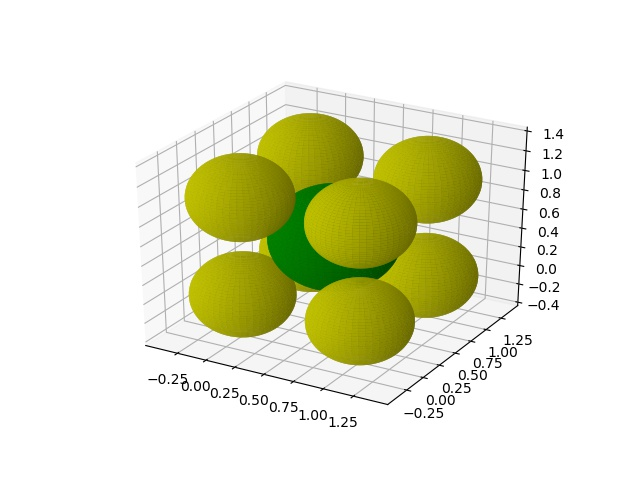
\includegraphics[width=\linewidth]{images/picturebcc.jpg}
        \caption{BCC unit cell schematic}
        \label{fig:sub1}
    \end{subfigure}
    \begin{subfigure}{0.5\textwidth}
        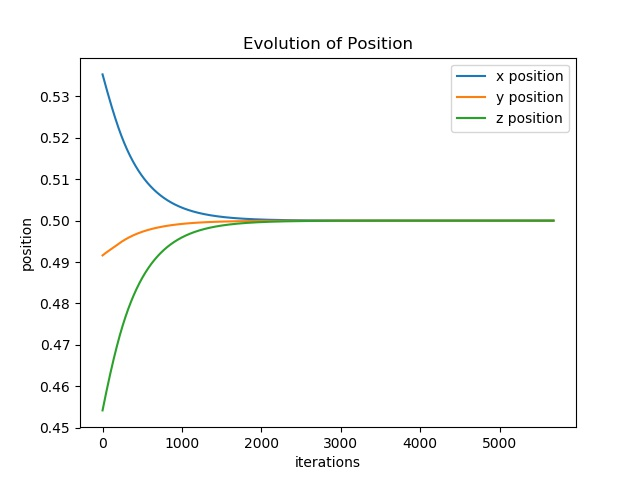
\includegraphics[width=\linewidth]{images/positionbcc.jpg}
        \caption{Evolution of position}
        \label{fig:sub2}
    \end{subfigure}
    \caption{BCC unit cell schematic and the evolution of $x,y,z$ positions of the center of the green sphere}
\end{figure}

\begin{figure}[h!]
    \begin{subfigure}{0.5\textwidth}
        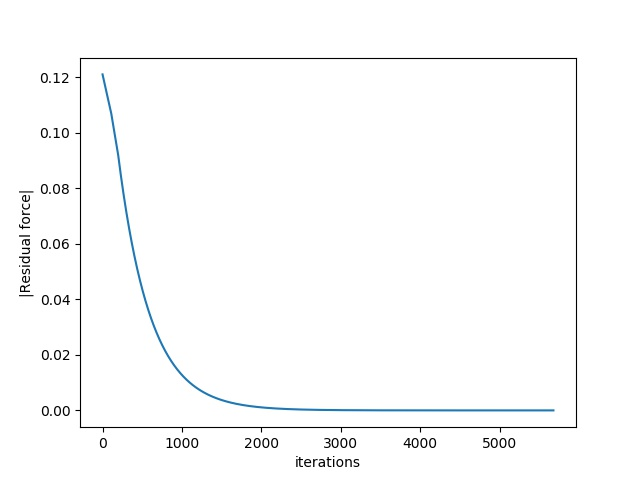
\includegraphics[width=\linewidth]{images/RF_bcc.jpg}
        \caption{Evolution of residual force on central droplet}
        \label{fig:sub1}
    \end{subfigure}
    \begin{subfigure}{0.5\textwidth}
        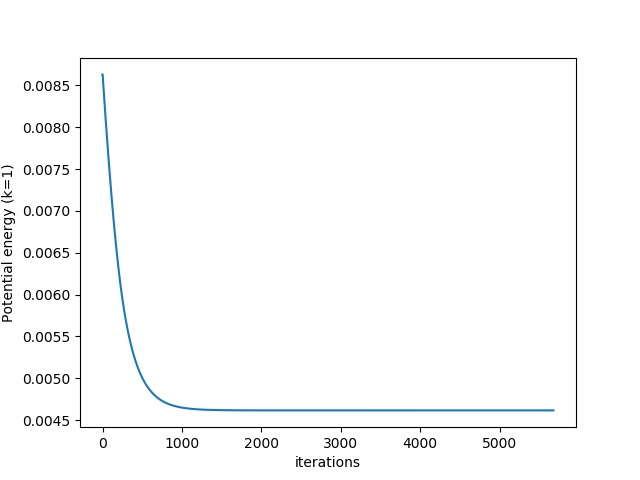
\includegraphics[width=\linewidth]{images/U_bcc.jpg}
        \caption{Evolution of potential energy of the system}
        \label{fig:sub2}
    \end{subfigure}
    \caption{Evolution of the potential energy and the residual force on the central droplet}
\end{figure}


\end{subsection}

\begin{subsection}{Cubic lattice 1: Simple Harmonic Potential}
\begin{figure}[h!]
    \begin{subfigure}{0.5\textwidth}
        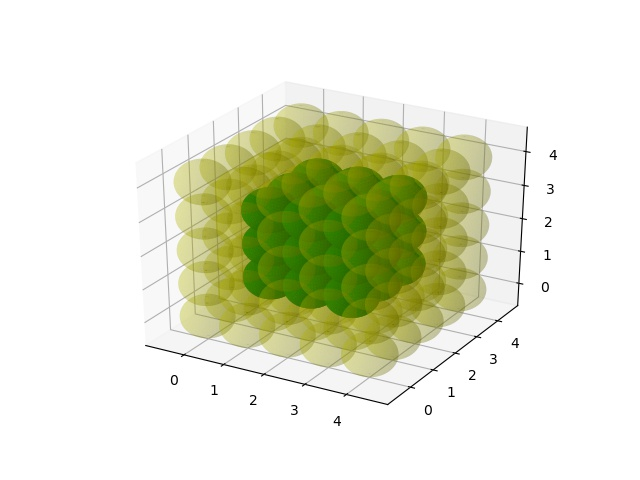
\includegraphics[width=\linewidth]{images/5x5x5_model.jpg}
        \caption{Schematic of the test case}
        \label{fig:sub1}
    \end{subfigure}
    \begin{subfigure}{0.5\textwidth}
        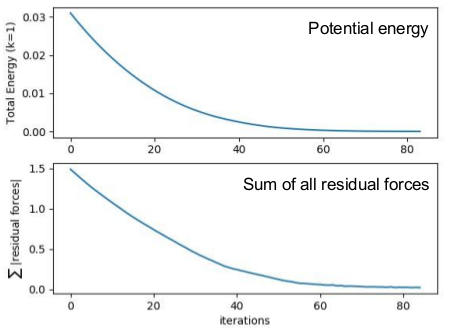
\includegraphics[width=\linewidth]{images/5by5by5_UandF.jpeg}
        \caption{Evolution of potential energy and sum of residual forces}
        \label{fig:sub2}
    \end{subfigure}
    \caption{Evolution of the potential energy and the residual force on the central droplet for Cubic Lattice 1}
\end{figure}
\noindent We now consider a more complicated case where we have 125 spheres of equal radii arranged on a $5 \times 5 \times 5$ cubic lattice with lattice parameter $a$ set equal to 1. The spheres are of radius 0.5 and are just touching each other in the equilibrium position. The expected minimum energy configuration is the one where the spheres are at the lattice sites, where the overlap between particles is zero and hence the forces vanish.\\ The outer layer of spheres is fixed and the $3 \times 3 \times 3$ cube at the center is displaced from the original positions and the particles return to the minimum energy configuration where the sum of magnitudes of residual forces goes to zero. 
\end{subsection}

\begin{subsection}{Cubic Lattice 2: Simple Harmonic Potential}
\begin{figure}[h!]
    \begin{subfigure}{0.5\textwidth}
        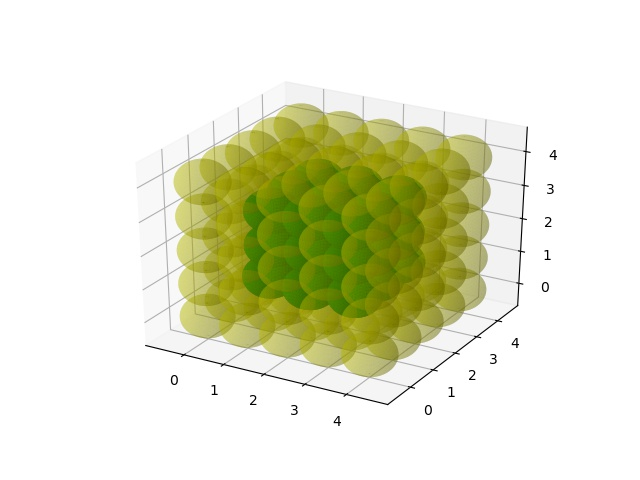
\includegraphics[width=\linewidth]{images/5x5x5_model_r6.jpg}
        \caption{Schematic of the test case}
        \label{fig:sub1}
    \end{subfigure}
    \begin{subfigure}{0.5\textwidth}
        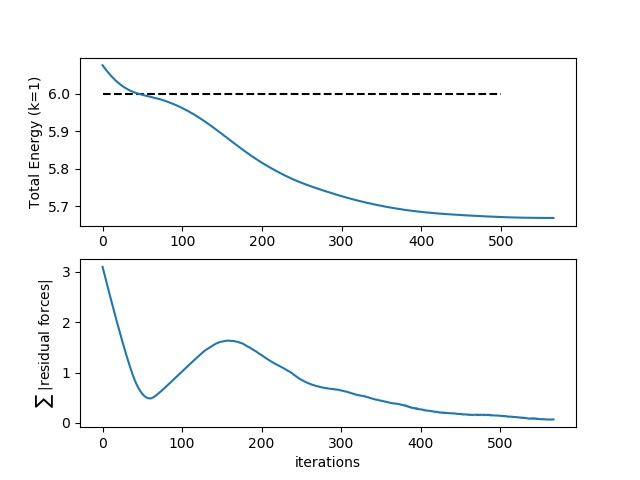
\includegraphics[width=\linewidth]{images/5by5by5_harmonic_r=6_UandF.jpeg}
        \caption{Evolution of potential energy and sum of residual forces}
        \label{fig:sub2}
    \end{subfigure}
    \caption{Evolution of the potential energy and the residual force on the central droplet for cubic lattice 2}
\end{figure}
\begin{figure}[h!]
    \centering
    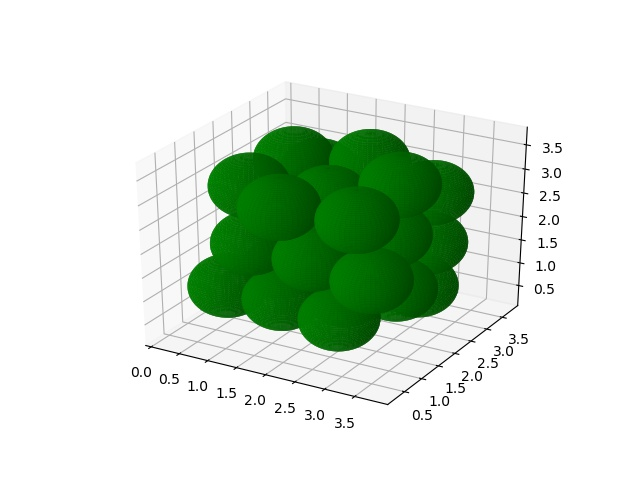
\includegraphics[width = 0.5\linewidth]{images/5x5x5_relaxed_r6.jpg}
    \caption{Relaxed positions of the droplets, not at the lattice sites, for cubic lattice 2}
    \label{fig:my_label}
\end{figure}
\noindent This case is similar to the $5 \times 5 \times 5$ cubic lattice (Cubic Lattice 1) with a radius larger than before so that the spheres now overlap in their equilibrium positions. The lattice parameter $a$ is set equal to 1 and the radius $r =0.6 \times a$. We expect that if disturbed from the mean positions, the particles will settle to the lattice sites, where the sum of forces is zero. Instead, it is observed that if the displacement of the particles is high initially, the systems finds a new minimum. In Figure (b), we see that the dashed line is the energy at lattice sites, and the system settles to the minima with lesser energy around 5.7 (energy units/k). The sum of forces as expected goes to zero at this minimum. This is another preferred packing with an energy lower than the lattice site configuration. It is important to note that we are looking for the nearest minimum  for our experimental data and not the global minimum. So depending on how big the errors in the positions are, the system may find a different minima which is undesirable. 
\end{subsection}

\begin{subsection}{Experimental Data: Simple Harmonic Potential}
\begin{figure}[h!]
    \centering
    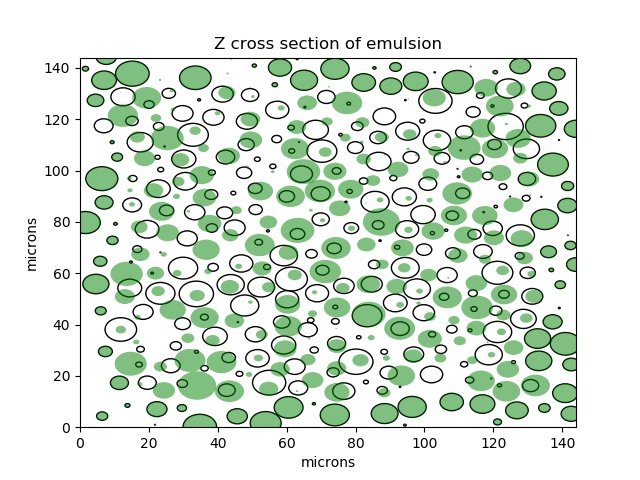
\includegraphics{images/relaxed_emulsion_harmonic.jpg}
    \caption{$z$ section of the initial state (green discs) and relaxed state(black circles) for the experimental modeled with a simple harmonic potential.}
    \label{fig:my_label}
\end{figure}
\par \noindent We assume that the forces in between the emulsion droplets follow a simple harmonic law which is proportional to the overlap. A $z$ cross section has been plotted to check what the initial and the relaxed state looks like. The boundary conditions are fixed boundaries as usual. As we observe, the relaxed state (black circles) looks very different from the initial image (green discs). This means that the system finds a minima very different from the nearest local minima that we desire.
This incorrect result was expected, since we know that the actual droplets do not interact through a simple harmonic force, and a different model needs to be used to model this. Hence, we use the Princen Model potential given in Section 4.6.
\end{subsection}

\newpage
\begin{subsection}{Experimental Data: Area-Dependent Potential}
\begin{figure}[h!]
    \begin{subfigure}{0.5\textwidth}
        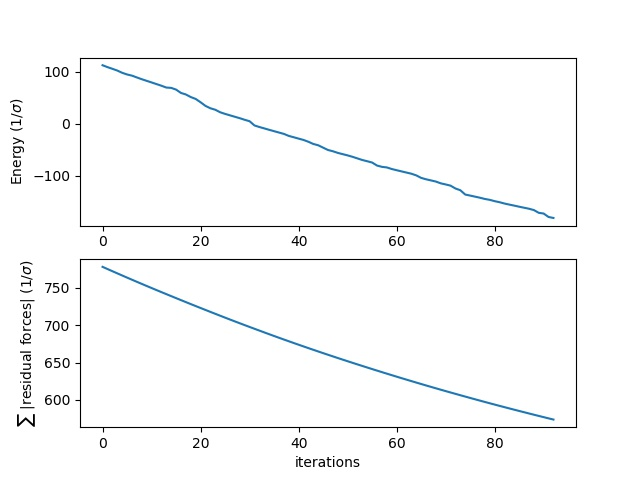
\includegraphics[width=\linewidth]{images/emulsion_UandF.jpeg}
        \caption{Evolution of potential energy and sum of residual forces}
        \label{fig:sub1}
    \end{subfigure}
    \begin{subfigure}{0.5\textwidth}
        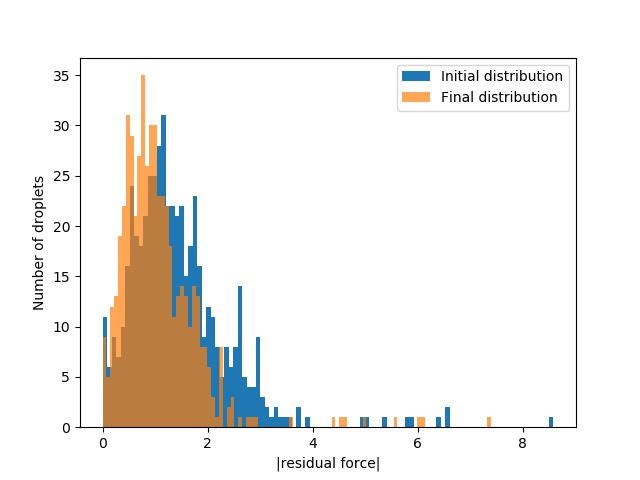
\includegraphics[width=\linewidth]{images/emulsion_residual_histogram.jpg}
        \caption{Initial and final distribution of residual forces}
        \label{fig:sub2}
    \end{subfigure}
    \caption{Evolution of the potential energy and the residual force on the central droplet}
\end{figure}
\par \noindent \newline We ran the gradient descent algorithm on the experimental data and saw that the descent stops after a few iterations, but the sum of residual forces is not zero. The histogram of the residual forces in the initial and final state also looks similar. The figure above shows one such failed trial for the experimental data. To resolve this, we tried to use an adaptive step size, which tried to take smaller steps assuming that the descent stops due to being stuck in a sharp valley, but this does not resolve the issue. \\\\
As a way to understand the problem, we tried to model the BCC and cubic lattice test cases using the area dependent potential for both mono-disperse and poly-disperse cases. All mono-disperse test cases worked, but the poly-disperse case works only for the BCC unit cell and not the $5\times5\times5$ cubic lattice. \\\\
To try to understand why the gradient descent stops for the poly-disperse case, we tried to plot the area dependent potential and the corresponding force in between the droplets.
\end{subsection}

\begin{subsection}{Understanding the Area-Dependent Potential}
\begin{figure}[h!]
    \begin{subfigure}{0.5\textwidth}
        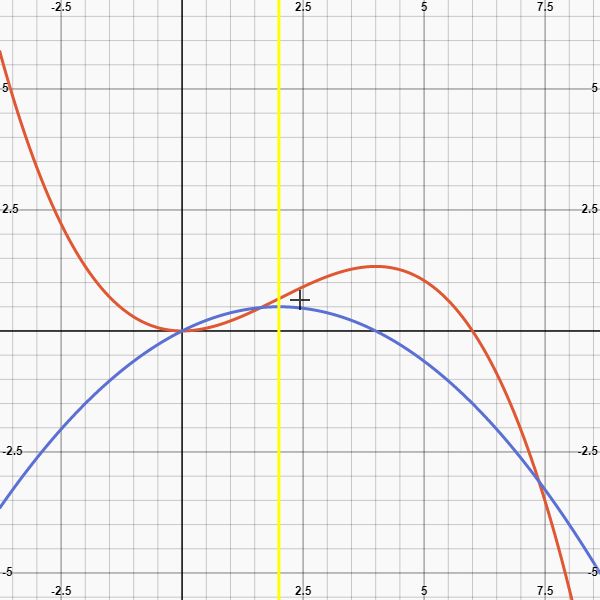
\includegraphics[width=0.9\linewidth]{images/potential_graph_1.png}
        \caption{$r_1 =1 ,  r_2 = 1$}
        \label{fig:sub1}
    \end{subfigure}
    \begin{subfigure}{0.5\textwidth}
        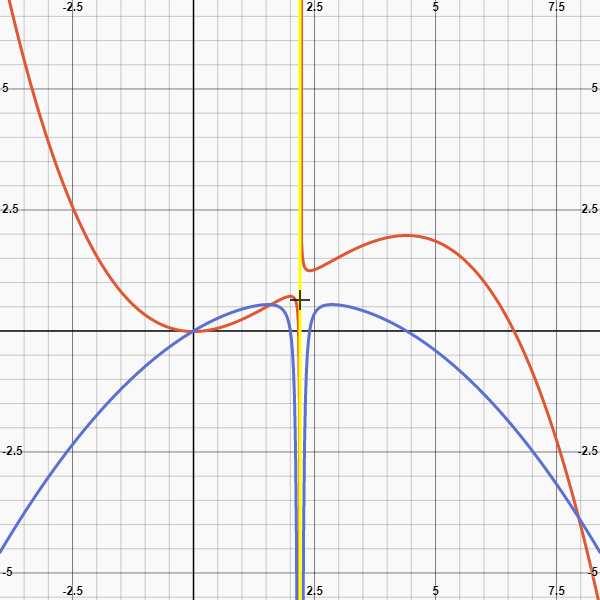
\includegraphics[width=0.9\linewidth]{images/potential_graph_2.png}
        \caption{$r_1 = 1 ,  r_2 = 1.2 $}
        \label{fig:sub2}
    \end{subfigure}
    \caption{Potential energy (\color{red}red line\color{}), magnitude of the residual force (\color{blue}blue line\color{}) and the position of the singularity (\color{yellow} yellow\color{}) \textit{(Courtesy: https://www.integral-calculator.com/)}}
\end{figure}
\par \noindent We find that there is a singularity in the potential and the force at $x = r_1 + r_2$, where $r_1$, $r_2$ are the radii of the droplets and $x$ in the overlap. This does not completely address the problem, because the overlaps on each iteration are much smaller than the overlap required to reach the singularity, however as discussed later, this may be the reason why the gradient descent does not converge to a configuration of minimum force. \\\\
From the plot of the potential, we can try to understand our results. For droplets with equal radii, the potential function is well-behaved except only at the singularity point. However, when the radii are unequal, the potential starts diverging before the singularity point. It may be the case that we are stuck at a point in the complicated landscape where the gradient descent takes us to an overlap greater than that required for the singularity and the gradient descent stops but the forces are not zero. This may be the reason why the mono-disperse cases work well, but there is a problem with poly-dispersity. 
\end{subsection}

\begin{subsection}{Experimental Data: Simple Cubic Potential}
We suspect that the singular behaviour of the potential causes the gradient descent to stop. With a view to address whether the problem arises due to the aforementioned reason, we try potentials which behave roughly like the area dependent potential, but do not have singularities. For this reason, we consider a cubic potential so that the force scales as the area which scales as square of the overlap.We try the simple cubic potential and the results are presented below. We see that the final distribution of forces is very close to zero as desired. A z cross section of the sample plotted below shows that the initial and final positions are quite different, but this performs better than the simple harmonic potential.
\begin{figure}[h!]
    \begin{subfigure}{0.5\textwidth}
        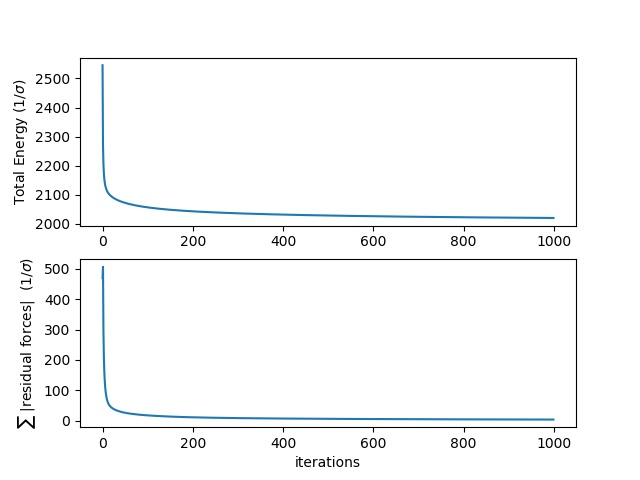
\includegraphics[width=\linewidth]{images/emulsion_cubic_UandF.jpeg}
        \caption{Evolution of potential energy and sum of residual forces}
        \label{fig:sub1}
    \end{subfigure}
    \begin{subfigure}{0.5\textwidth}
        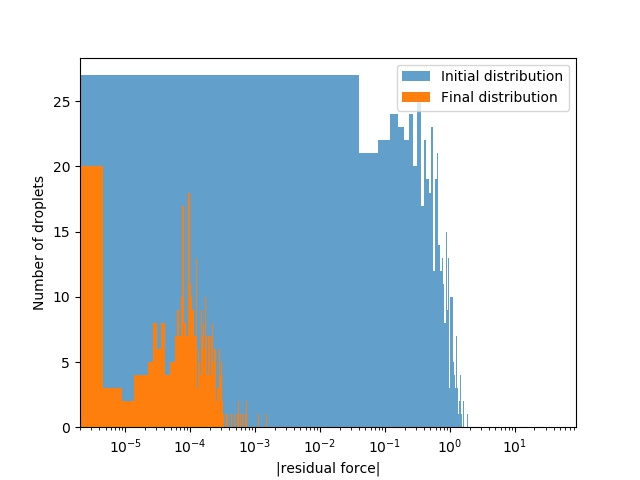
\includegraphics[width=\linewidth]{images/emulsion_cubic_residual_histogram.jpg}
        \caption{Initial and final distribution of residual forces}
        \label{fig:sub2}
    \end{subfigure}
    \caption{Evolution of the potential energy and the residual force for the simple cubic potential}
\end{figure}
\begin{figure}[h!]
    \centering
    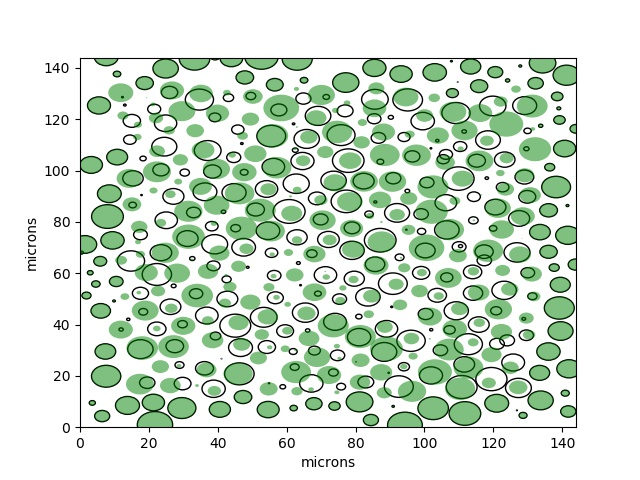
\includegraphics[width=0.6\linewidth]{images/emulsion_cubic_cross_section.jpg}
    \caption{$z$ section of the initial state (green discs) and relaxed state(black circles) for the experimental modeled with a simple cubic potential.}
    \label{fig:my_label}
\end{figure}
\end{subsection}

\newpage
\begin{subsection}{Experimental Data: Anisotropic Cubic Potential}
As we see that the cubic potential does not do too well, we introduce the anisotropic factor $\Tilde{r} = \frac{r_1 r_2}{r_1 + r_2}$ and find that forces again go to zero, but with this potential we get better results for the relaxed state, which appears to be quite close to the initial configuration as seen by the cross section.
\begin{figure}[h!]
    \begin{subfigure}{0.5\textwidth}
        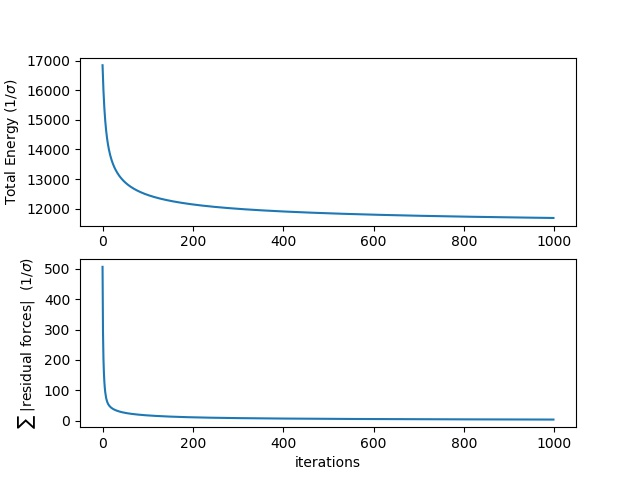
\includegraphics[width=\linewidth]{images/emulsion_cubic_anisotropic_UandF.jpeg}
        \caption{Evolution of potential energy and sum of residual forces}
        \label{fig:sub1}
    \end{subfigure}
    \begin{subfigure}{0.5\textwidth}
        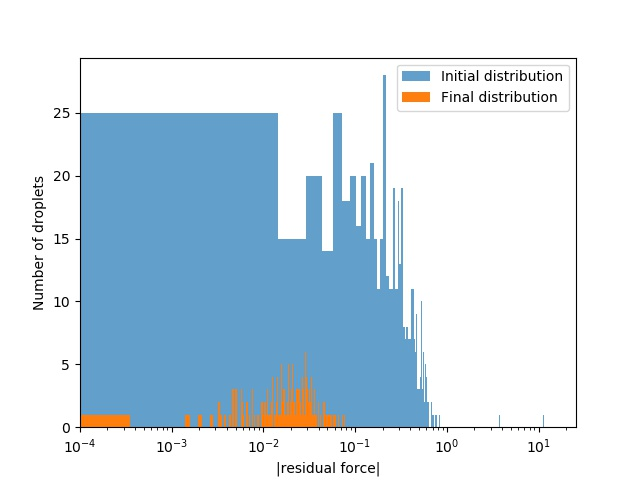
\includegraphics[width=\linewidth]{images/emulsion_cubic_anisotropic_residual_histogram.jpg}
        \caption{Initial and final distribution of residual forces}
        \label{fig:sub2}
    \end{subfigure}
    \caption{Evolution of the potential energy and the residual force on the central droplet for the anisotropic cubic potential}
\end{figure}
\begin{figure}[h!]
    \centering
    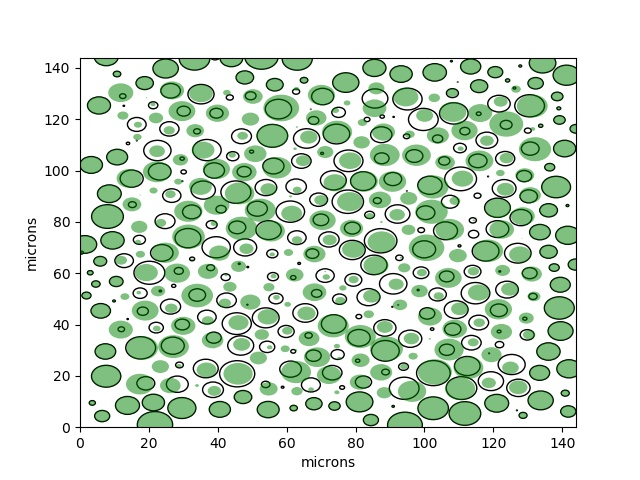
\includegraphics[width=0.6\linewidth]{images/emulsion_cubic_anisotropic_cross_section.jpg}
    \caption{$z$ section of the initial state (green discs) and relaxed state(black circles) for the experimental modeled with the anisotropic cubic potential.}
    \label{fig:my_label}
\end{figure}
\par \noindent We can see that this has already started to look much better as the particles have not moved  from their positions by a lot, and we see that the residual forces have vanished. So we conclude that there is indeed a problem with the potential that we are using. 

\end{subsection}

\end{section}
%%%%%%%%%%%%%%%%%%%%%%%%%%%%%%%%%%

\begin{section}{Discussion and Future Directions}
We implemented the gradient descent algorithm and found that it was working on all test cases for the simple harmonic potential. After proceeding to work with the area dependent potential, we discovered that for the complicated setups such as the cubic lattice and the real data, the gradient descent stopped at a point where the residual forces were not zero, but we could not lower the energy further. The reason for this was hypothesized to be due to the singularities in the potential at large overlaps. Although these overlaps are never reached for any of the cases, it seems that in a complex picture, the singularities play a role due to the energy being a very complicated function of the positions and radii of the droplets in the sample. \\\\
So far, we have only tried to implement the gradient descent by changing the positions of the centers. It is also possible that the errors arise from the radii, and corrections must be made simultaneously to the positions and the radii. However, thich code will prove useful to cases where we want to see how a system relaxes to its equilibrium position given the interactions in between the particles.\\\\
Studying the mechanical properties of the emulsion is the primary goal and we should try to construct the Hessian matrix once the equilibrium positions are obtained. A primary calculation of the vibrational modes should be done before correcting the data, as see how much the vibrational spectrum varies from the spectrum obtained from the relaxed picture. If we notice that it does not vary significantly, we may as well calculate the vibrational modes without correction. 

\end{section}

%%%%%%%%%%%%%%%%%%%%%%%%%%%%%%%%%%
\bibliographystyle{unsrt}
\bibliography{bib_file}
\end{document}




